%!TEX root = ../main.tex

\chapter{L'imagerie \glsentryshort{stem}-\glsentryshort{eels} : présentation et problématiques}
\label{ch-chapter_1}

    \dochaptoc
    \graphicspath{{img/chapitre1/}}

    \section{Présentation de la microscopie \glsentryshort{stem}}

    L'ensemble du travail de thèse présenté dans ce manuscrit se base sur des données issues d'un système de microscopie appelé microscope électronique en transmission à balayage ou encore \acf{stem}\glsunset{stem}. Ce système utilise un faisceau d'électrons pour illuminer un échantillon et obtenir ainsi un agrandissement de la zone à étudier, il s'agit donc d'un microscope électronique. Nous allons commencer par positionner le \gls{stem} au sein de la microscopie électronique pour ensuite décrire plus précisément son fonctionnement.

    \subsection{La microscopie électronique}

    Un microscope électronique se compose classiquement d'une source d'électrons (aussi appelée canon), de lentilles électromagnétiques permettant de focaliser le faisceau de particules sur l'échantillon et d'un détecteur. Les types de microscopes électroniques se différencient par la façon dont l'échantillon est illuminé et par la position du détecteur. Nous y trouvons donc :
    \begin{itemize}
    	\item la microscopie électronique en transmission (aussi appelée \gls{tem}) pour laquelle le faisceau d'électrons illumine l'ensemble de l'échantillon et le traverse pour être ensuite analysé,
    	\item la microscopie \gls{stem} pour laquelle le faisceau d'électrons est focalisé sur un point de l'échantillon et le traverse pour être ensuite analysé,
    	\item la microscopie électronique à balayage (aussi appelée \gls{sem}) pour laquelle le faisceau d'électrons est focalisé sur un point de l'échantillon et le détecteur positionné en amont capte des électrons secondaires ayant été déviés.
    \end{itemize}
    La \cref{fig-chap2-micros-electron} propose un schéma simplifié de chacune de ces configurations. Toutes ces modalités permettent l'acquisition d'une image contrastée 2D qui est une représentation agrandie de l'échantillon.

    \begin{figure*}[t!]
       	\centering
       	\subfigure[Légende]{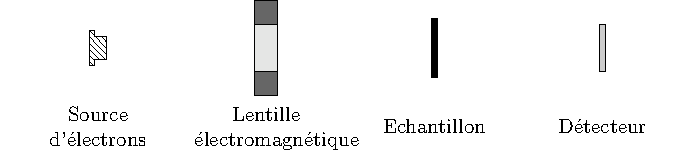
\includegraphics[]{img/chapitre1/figure1/subfig-a/electronic-legend.pdf}
       	}\\
       	\subfigure[Le microscope \gls{tem}]{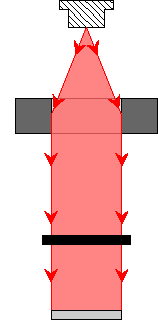
\includegraphics[]{img/chapitre1/figure1/subfig-b/electronic-tem.pdf}}
       	\hspace*{2cm}
       	%
       	\subfigure[Le microscope \gls{stem}]{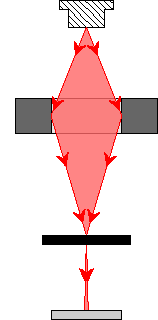
\includegraphics[]{img/chapitre1/figure1/subfig-c/electronic-stem.pdf}}
       	\hspace*{2cm}
       	%
       	\subfigure[Le microscope \gls{sem}]{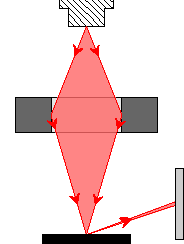
\includegraphics[]{img/chapitre1/figure1/subfig-d/electronic-sem.pdf}}
       	%
           \vspace{1em}
       	\caption{Schéma de principe des différents types de microscopie électronique.%
               \protect\label{fig-chap2-micros-electron}}
   \end{figure*}

    Les microscopes \gls{stem} et \gls{sem} se différencient du \gls{tem} puisque le faisceau balaye l'échantillon ligne par ligne au lieu de l'illuminer entièrement. Il en résulte que ces premiers sont destinés principalement à la \emph{spectroscopie}, \ie{} à l'acquisition d'un spectre pour chaque position spatiale. Les données peuvent alors être représentées comme un cube ayant deux dimensions spatiales et une dimension spectrale. Les applications classiques de ces systèmes sont la détection et cartographie d'éléments chimiques présents dans l'échantillon (\cf{} \cref{sec-exploitation-eels}). Le \gls{tem} est davantage utilisé en \emph{imagerie} pour représenter l'échantillon sans analyse chimique possible.

    La suite de ce manuscrit se focalisera sur la microscopie \gls{stem} qui est le centre de notre étude. C'est pourquoi le principe physique de la microscopie en transmission est évoqué à la \cref{subsec-principe-physique-tem} et les modalités d'acquisition classiques sont présentées à la \cref{subsec-modalitees-stem}. A cette fin, un schéma plus détaillé de ce système et de ses modalités d'acquisition est donné à la \cref{fig-chap2-stem-detail}. Enfin, le contenu technique de ce chapitre s'inspire des livres de Egerton~\cite{egerton2011electron} et de Colliex~\cite{colliex1998microscopie} et nous renvoyons les lecteurs curieux à ces ouvrages pour de plus amples informations.

    \begin{figure*}[htbp]
    	\centering
    	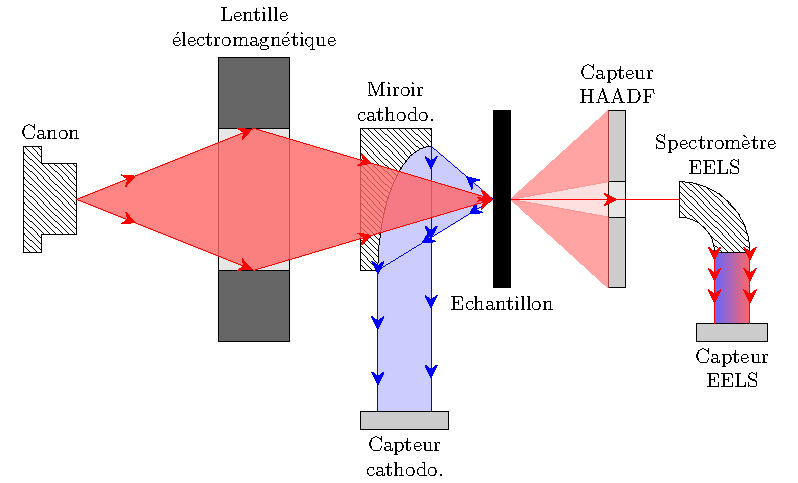
\includegraphics[]{img/chapitre1/figure2/stem-detail.pdf}
    	\caption{Un schéma de principe détaillé du \gls{stem}.
        	\protect\label{fig-chap2-stem-detail}}
    \end{figure*}

    \subsection{Principe de la microscopie en transmission}\label{subsec-principe-physique-tem}

    La microscopie en transmission étudie les interactions physiques entre un faisceau d'électron et la matière qu'il traverse. Pour ce faire, un canon fournit une certaine énergie cinétique à un faisceau d'électrons, celui-ci est alors focalisé en un point de l'échantillon à l'aide de lentilles électromagnétiques. Afin que ce faisceau \emph{traverse} l'échantillon, plusieurs conditions doivent être réunies :
    \begin{enumerate}[label=(\alph*)]
    	\item l'énergie cinétique des électrons doit être suffisante (typiquement 100keV, correspondant à une vitesse d'environ 2/3 de la vitesse de la lumière),
    	\item l'échantillon doit être suffisamment fin (typiquement 100nm pour un faisceau de 100keV).
    \end{enumerate}
    Dans ces conditions, les électrons traversent l'échantillon sans subir d'absorption ni de réflexion notoire. A noter qu'il est nécessaire de faire le vide dans le corps du microscope afin d'éviter toute collision entre le faisceau et les molécules d'air. Dès lors, deux types d'interactions électron-atome vont avoir lieu au sein de l'échantillon, schématisées aux figures~\ref{fig-chap2-interactions-a} et \ref{fig-chap2-interactions-b}.

    Tout d'abord, l'électron incident interagit avec le noyau de l'atome fortement chargé par une attraction électrostatique d'autant plus intense que celui-ci s'approche du noyau, comme le montre la figure~\ref{fig-chap2-interactions-a}. Cette interaction est appelée diffusion élastique puisqu'il n'y a pas de perte d'énergie cinétique. Cela dit, la majorité des électrons traversent l'atome suffisamment loin du noyau pour être peu déviés et la déviation angulaire associée est de l'ordre du demi-degré (10\;mrad).
    
    D'autre part, l'électron incident traversant le nuage électronique peut interagir avec les électrons le constituant et leur communique de l'énergie, \ie\ dans le modèle atomique les faire passer d'un niveau à un autre, ou même les expulser complètement de façon à transformer l'atome initialement neutre en ion. La perte  d'énergie subie par l'électron incident est ainsi gagnée par l'électron de la cible, comme montré sur les figures~\ref{fig-chap2-interactions-b} et \ref{fig-chap2-interactions-c}. Ce type d'interaction mettant en jeu un transfert d'énergie est appelé \emph{diffusion inélastique}. La déviation angulaire est en général sensiblement plus faible que dans le cas de la diffusion élastique et les électrons concernés sont concentrés dans un domaine angulaire restreint (de l'ordre de 0.1 à 1\;mrad).
    
    Pour résumer, les électrons traversant l'échantillon peuvent être déviés de leur trajectoire par diffusion élastique ou inélastique et une partie d'entre eux ont perdu de l'énergie cinétique par diffusion inélastique. Les modalités d'acquisition du \gls{stem} se basent sur la détection de ces deux effets.

    \begin{figure}
    	\centering
    	\subfigure[Diffusion élastique]{
    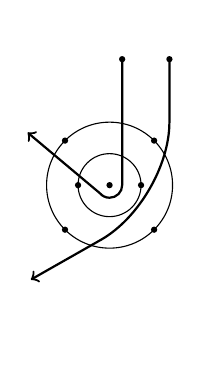
\begin{tikzpicture}[scale=0.4]
        \clip (-2.6, -5) rectangle (2.5, 5);
        \coordinate (O) at (0, 0);
        \coordinate (A) at (0.4, 4);
        \coordinate (B) at (1.9, 4);

        % Circles
        \draw (O) circle (1cm);
        \draw (O) circle (2cm);

        % Central atom
        \fill[black] (O) circle (0.1cm);

        % Atoms on layers # 1
        \fill[black] (0:1) circle (0.1cm);
        \fill[black] (180:1) circle (0.1cm);

        % Atoms on layers # 2
        \fill[black] (45:2) circle (0.1cm);
        \fill[black] (90+45:2) circle (0.1cm);
        \fill[black] (180+45:2) circle (0.1cm);
        \fill[black] (270+45:2) circle (0.1cm);

        % Incident atoms
        \fill[black] (A) circle (0.1cm);
        \fill[black] (B) circle (0.1cm);

        \draw[->, thick ] (A) -- (0.4, 0) arc (0:-140:0.4) -- ++ (140:3);
        \draw[->, thick, rounded corners=1cm ] (B) -- ++(0, -4.5) -- (-2.5, -3);

    \end{tikzpicture}
    \label{fig-chap2-interactions-a}
}\quad
\subfigure[Diffusion inélastique]{\small
    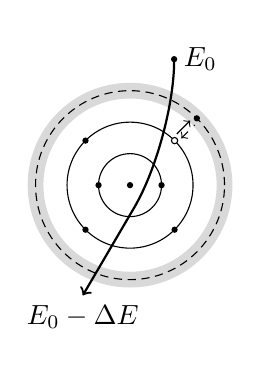
\begin{tikzpicture}[scale=0.4]
        \clip (-3.25, -5) rectangle (3.25, 5);

        \coordinate (O) at (0, 0);
        \coordinate (A) at (1.4, 4);

        % Circles
        \draw (O) circle (1cm);
        \draw (O) circle (2cm);

        % Central atom
        \fill[black] (O) circle (0.1cm);

        % Atoms on layers # 1
        \fill[black] (0:1) circle (0.1cm);
        \fill[black] (180:1) circle (0.1cm);

        % Atoms on layers # 2
        \filldraw [draw=black, fill=white] (45:2) circle (0.1cm);
        \fill[black] (90+45:2) circle (0.1cm);
        \fill[black] (180+45:2) circle (0.1cm);
        \fill[black] (270+45:2) circle (0.1cm);

        % Layer # 3
        \fill [black!15, even odd rule] (O) circle (3.25cm) circle (2.75cm);
        \draw [densely dashed] (O) circle (3cm);

        % Incident atoms
        \fill[black] (A) circle (0.1cm);
        \draw (A) node [right] {$E_0$};
        \draw[->, thick, rounded corners=1cm ] (A) -- ++(0, -2.55) -- (-1.5, -3.5) node [below] {$E_0-\Delta E$};

        % Other atom and arrows
        \fill [black] (45:3) circle (0.1cm);
        \draw [->, rotate=45] (2.2, 0.1) -- ++ (0.6, 0);
        \draw [<-, dashed, rotate=45] (2.2,- 0.1) -- ++ (0.6, 0);

    \end{tikzpicture}
    \label{fig-chap2-interactions-b}
}\quad
\subfigure[Transition énergétique en diffusion inélastique]{\small
    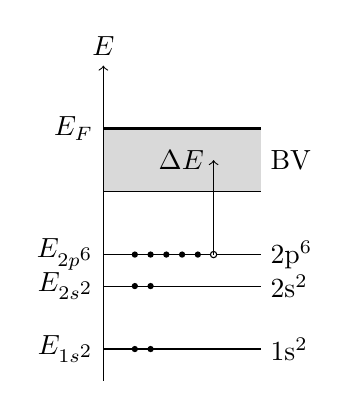
\begin{tikzpicture}[scale=0.4]
        %\clip (-3.25, -4) rectangle (3.25, 4);

        % horiz. lines
        \draw (0, 1) node [left] {$E_{\text{1s\textsuperscript{2}}}$} -- (5, 1) node [right] {1s\textsuperscript{2}};
        \draw (0, 3) node [left] {$E_{\text{2s\textsuperscript{2}}}$} -- (5, 3) node [right] {2s\textsuperscript{2}};
        \draw (0, 4) node [left] {$E_{\text{2p\textsuperscript{6}}}$} -- (5, 4) node [right] {2p\textsuperscript{6}};

        % Valance band
        \fill [black!15] (0, 6) -- (5, 6) -- (5, 8) -- (0, 8) -- cycle;
        \draw (0, 6) -- (5, 6);
        \draw [thick] (0, 8) node [left] {$E_F$} -- (5, 8);
        \draw (5, 7) node [right] {BV};

        % Left axis
        \draw [->] (0, 0) -- (0, 10) node[above] {$E$};

        % Atoms
        \foreach \n in {1, 1.5}{\fill [black] (\n, 1) circle (0.1cm);}
        \foreach \n in {1, 1.5}{\fill [black] (\n, 3) circle (0.1cm);}
        \foreach \n in {1, 1.5, ..., 3}{\fill [black] (\n, 4) circle (0.1cm);}

        % Moved atom
        \fill [draw=black, fill=white] (3.5, 4) circle (0.1cm);
        \draw [->] (3.5, 4) -- (3.5, 7) node [left] {$\Delta E$};

    \end{tikzpicture}
    \label{fig-chap2-interactions-c}
}

        \vspace{1em}
    	\caption{Une représentation classique de la diffusion électronique inspirée de~\cite{egerton2011electron} et de \cite{colliex1998microscopie}.
        \subref{fig-chap2-interactions-a} Diffusion élastique : l'électron incident est dévié par interaction électrostatique avec le noyau. 
        \subref{fig-chap2-interactions-b} Diffusion inélastique : l'électron incident perd de l'énergie cinétique en faveur d'un électron du nuage atomique.
        \subref{fig-chap2-interactions-c} Représentation des niveaux d'énergie de l'atome. La diffusion inélastique permet à l'un des électrons du nuage électronique de passer dans un état d'énergie supérieur, en bande de valence ou au-delà.  %  
            \protect\label{fig-chap2-interactions}}
    \end{figure}


    \subsection{Les modalités d'acquisition en microscopie \glsentryshort{stem}}\label{subsec-modalitees-stem}

    Le \gls{stem} permet entres autre trois modalités d'acquisition : la cathodoluminescence, l'acquisition fond noir angulaire à grand angle (ou encore \gls{haadf}) et la spectroscopie par perte d'énergie (ou encore \gls{eels}). La \cref{fig-chap2-stem-detail} sert de support pour situer les capteurs correspondant au sein du \gls{stem}.

    \paragraph*{Cathodoluminescence.} Pour certains échantillons, le faisceau incident produit un phénomène de fluorescence dépendant de la nature de l'échantillon et de ses défauts. La technique consistant à acquérir ce signal et à l'étudier s'appelle \emph{la cathodoluminescence}. Le flux lumineux est recueilli à l'aide d'un miroir situé en amont de l'échantillon puis envoyé vers un spectromètre qui procède à la mesure.

    \paragraph{\gls{haadf}.} Le faisceau incident se situe dans l'axe optique de l'appareil et une grande partie des électrons traversent l'échantillon en demeurant dans cet axe, la diffusion élastique est alors négligeable. Néanmoins, une partie des électrons sont significativement déviés de l'axe optique en sortie.  Un capteur annulaire placé en aval de l'échantillon capte ces électrons et délivre un signal proportionnel. Cette technique appelée \gls{haadf} permet de fournir une image 2D de l'échantillon. Deux exemples d'acquisition \gls{haadf} sont fournis à la \cref{fig-chap2-haadf-ex}.

    \begin{figure}%[htbp]
    	\centering
    	\subfigure[\label{fig-chap2-haadf-ex-a}Acquisition basse-résolution]%
            {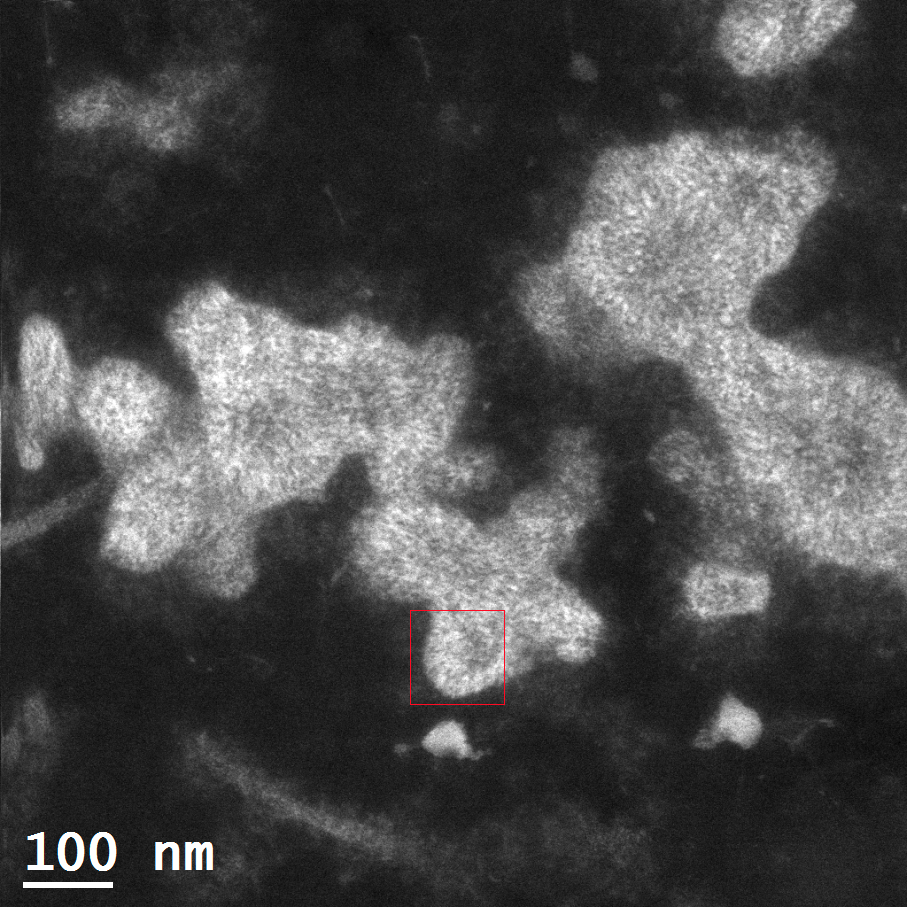
\includegraphics[height=0.25\textwidth]{img/chapitre1/figure4/haadf-LR.png}}
        \hspace{1em}
        \subfigure[\label{fig-chap2-haadf-ex-b}Acquisition haute-résolution]%
            {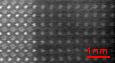
\includegraphics[height=0.25\textwidth]{img/chapitre1/figure4/haadf-HR-sc.png}}
     	%
        \caption{\protect\label{fig-chap2-haadf-ex}Exemples d'acquisitions \gls{haadf}. L'acquisition basse-résolution~\protect\subref{fig-chap2-haadf-ex-a} est de taille micrométrique  tandis que l'acquisition haute-résolution~\protect\subref{fig-chap2-haadf-ex-b} est de taille nanométrique.}
     \end{figure}


    \paragraph*{\gls{eels}.} Comme expliqué précédemment, certains électrons traversant l'échantillon  perdent une partie de leur énergie initiale par diffusion inélastique. Afin de détecter ces pertes, le faisceau demeuré dans l'axe optique frappe un spectromètre séparant les électrons en fonction de leur énergie. Une caméra CCD permet de compter, pour chaque position sur l'échantillon, la quantité d'électrons ayant conservé une énergie donnée. \`A chaque position spatiale correspond alors un spectre de perte d'énergie, les images \gls{eels} sont d'ailleurs également appelées \emph{spectre-image}. La microscopie \gls{eels} constitue le centre de cette étude, c'est pourquoi nous allons détailler ces données et leurs propriétés dans la section suivante.


    \section{Propriétés des données \glsentryshort{eels}}\label{sec-prop-eels}

    \begin{figure}[t]
        \centering
        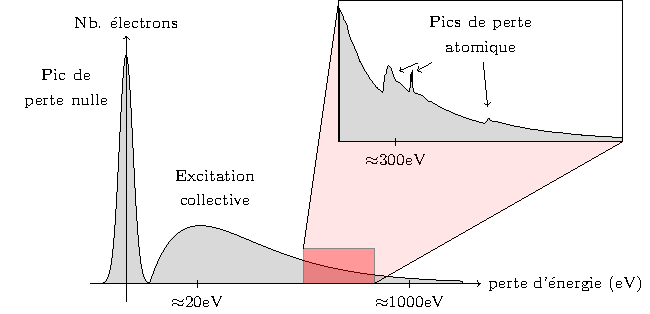
\includegraphics[]{img/chapitre1/figure5/eels-spectrum-shape.pdf}
        \caption{Représentation d'un spectre \gls{eels}.
            \protect\label{fig-chap2-eels-spectrum-shape}}
    \end{figure}

    \subsection{Caractéristiques spectrales} La forme générique d'un spectre \gls{eels} est représentée à la \cref{fig-chap2-eels-spectrum-shape} et affiche le nombre d'électrons ayant traversé l'échantillon en fonction de l'énergie perdue après la traversée (on parle de \emph{canal} pour désigner l'indice associé à une perte d'énergie). Il se compose de trois parties :
    \begin{itemize}
    	\item un pic de perte nulle qui correspond à l'ensemble des électrons ayant traversé l'échantillon sans interagir avec lui, et donc sans avoir perdu d'énergie,
    	\item un pic plus étalé correspondant à une excitation collective de la bande de valence,
    	\item une zone d'intérêt où un ensemble de pics caractéristiques (appelés \emph{seuils}) émergent du fond décroissant.
    \end{itemize}
    L'information utile est portée par la position, la forme et l'amplitude des seuils. En effet, la position d'un seuil permet de déterminer l'élément présent dans l'échantillon tandis que son amplitude nous renseigne sur son abondance pour chaque position spatiale. Enfin, la forme du seuil peut varier suivant la configuration électronique de l'élément étudié.
    %
    \`A titre d'exemple, les seuils généralement rencontrés dans nos données se situent à des pertes d'énergie de l'ordre de \np{500} à \np[eV]{1000} (pour rappel, une énergie typique en amont de l'échantillon est \np[keV]{100}).
    %
    Des exemples réels de spectres sont donnés à la \cref{fig-chap2-eels-real-spectra-figure}.


    \begin{normalfigure*}[p]
        \centering
        \subfigure[La position des spectres]{
            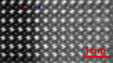
\includegraphics[width=0.3\textwidth]{img/chapitre1/figure6/eels_spectra_haadf-sc.png}
            \label{fig-chapitre2-real-eels-haadf}
        }\\
        \subfigure[Les spectres pour les trois positions]{
            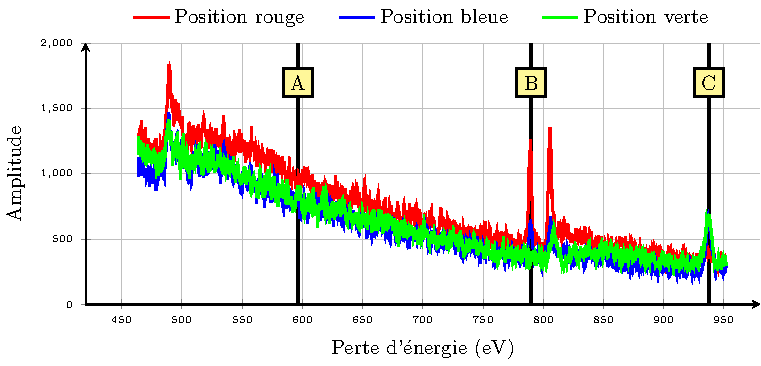
\includegraphics[]{img/chapitre1/figure6/eels_spectra.pdf}
            \label{fig-chapitre2-real-eels-spectra}
        }\\
        %
        \subfigure[Bande A]{% $\mathrm{O-K}$
            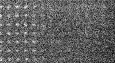
\includegraphics[width=0.3\textwidth]{img/chapitre1/figure6/eels_spectra_band_410.png}
            \label{fig-chapitre2-real-eels-bandA}
        }
        \hspace*{0.5cm}
        %
        \subfigure[Bande B ($\mathrm{La-M}_{4, 5}$)]{
            
\includegraphics[width=0.3\textwidth]{img/chapitre1/figure6/eels_spectra_band_1001.png}
            \label{fig-chapitre2-real-eels-bandB}
        }
        \hspace*{0.5cm}
        %
        \subfigure[Bande C ($\mathrm{Nd-M}_{4, 5}$)]{
            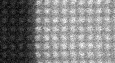
\includegraphics[width=0.3\textwidth]{img/chapitre1/figure6/eels_spectra_band_1465.png}
            \label{fig-chapitre2-real-eels-bandC}
        }

        \caption{Exemple réel de spectre-image \gls{eels}. La figure~\protect\subref{fig-chapitre2-real-eels-haadf} représente l'image \gls{haadf} de l'acquisition et trois positions en rouge, bleu et vert. Les spectres acquis en ces trois positions sont représentés à la figure~\protect\subref{fig-chapitre2-real-eels-spectra}. Enfin, les images à trois niveaux de perte d'énergie (notées A, B et C sur la figure~\subref{fig-chapitre2-real-eels-spectra}) sont représentées aux figures~\subref{fig-chapitre2-real-eels-bandA} à \subref{fig-chapitre2-real-eels-bandC}. Les bandes B et C correspondent respectivement aux signatures $\mathrm{La-M}_{4, 5}$ et $\mathrm{Nd-M}_{4, 5}$ tandis que la bande A ne correspond à aucune signature.
            \protect\label{fig-chap2-eels-real-spectra-figure}}
    \end{normalfigure*}

    \begin{figure*}[]
        \centering
        \subfigure[\label{fig-seuil-a}]{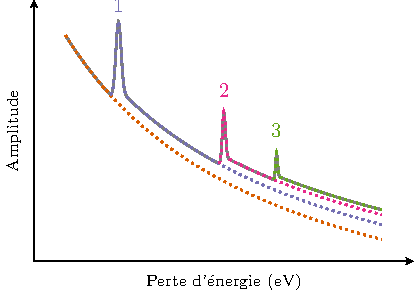
\includegraphics[]{img/chapitre1/figure6-bis/seuils.pdf}}
        \hspace{1em}
        \subfigure[\label{fig-seuil-b}]{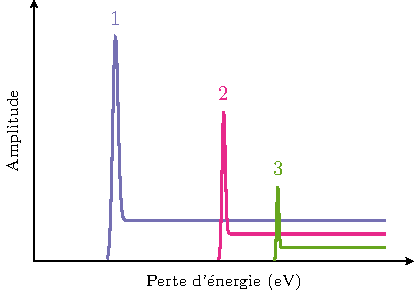
\includegraphics[]{img/chapitre1/figure6-bis/seuils-2.pdf}}
        \caption{Visualisation des effets des seuils successifs sur le spectre. La figure~\subref{fig-seuil-a} représente un spectre constitué de trois seuils. La figure~\subref{fig-seuil-b} représente les effets isolés de chacun des trois seuils. 
            \protect\label{fig-decroissance-spectre}}
    \end{figure*}

    La forme d'un seuil ne se limite pas au seul pic pour des raisons physiques, mais elle se poursuit au-delà puisque l'électron éjecté par diffusion inélastique peut avoir tout un continuum d'énergie au-delà de l'énergie de Fermi. Plus précisément, la forme du seuil varie en fonction des atomes présents au voisinage de l'élément d'intérêt, on parle de \emph{structure fine}.
    
    Le spectre acquis se décompose en un fond continu représentant l'ensemble des contributions des seuils antérieurs et d'autres phénomènes physiques, généralement modélisé par une exponentielle décroissante, et en un ensemble de seuils d'intérêt situés dans la fenêtre d'observation. La \cref{fig-decroissance-spectre} illustre cela. Cette décomposition est à la base des techniques de cartographie que l'on décrira en \cref{sec-exploitation-eels}.
    

    \subsection{Caractéristiques spatiales} En microscopie, comme pour beaucoup de systèmes d'imagerie, la caractéristique principale est le pouvoir séparateur de l'instrument, aussi appelé résolution. En microscopie \gls{stem}, celle-ci est principalement limitée par la taille de la sonde électronique (typiquement 1~nm) et par les aberrations sphériques (un correcteur permet de descendre à 0.1~nm). D'autre part, la résolution, telle qu'entendue en traitement du signal\footnote{La résolution de l'image correspond au nombre de pixels par unité de longueur. Pour éviter toute ambiguïté, on désignera par la suite la résolution de l'instrument par le terme \guillemets{pouvoir séparateur}, plus explicite.}, est choisie par l'expérimentateur en fonction de la distance parcourue par la sonde entre deux acquisitions. Cependant, en imagerie \gls{eels}, la taille de l'image excède rarement $10^5$ pixels pour limiter le temps d'acquisition et éviter de détériorer l'échantillon (comme décrit à la section~\ref{sec-ech-sensibles}). Par conséquent, deux situations apparaissent~:
    \begin{itemize}
        \item l'expérimentateur étudie des structures spatiales étendues (typiquement 100~nm) et est obligé de limiter la résolution, les images sont alors basse-résolution (\cf{} \cref{fig-chap2-haadf-ex-a}),
        \item l'expérimentateur étudie des réseaux atomiques très localisés (typiquement quelques nanomètres) et la résolution est limitée par l'instrument, les images sont alors haute-résolution (\cf{} \cref{fig-chap2-haadf-ex-b}).
    \end{itemize}
    Enfin, il faut noter que la structure spatiale est plus ou moins visible selon le canal considéré dans l'image \gls{eels}. Par exemple, la \cref{fig-chapitre2-real-eels-bandA} correspond à une zone du spectre où aucun contraste n'apparaît clairement, il en résulte que l'image est fortement bruitée. A contrario, les images situées sur des seuils particuliers du spectre sont moins bruitées et mettent clairement en évidence la position des éléments concernés, comme pour les \cref{fig-chapitre2-real-eels-bandB,fig-chapitre2-real-eels-bandC}.  La cartographie des éléments présents dans l'échantillon requiert des méthodes particulières afin de soustraire la contribution du fond continu, comme nous le verrons à la \cref{sec-exploitation-eels}.

    \subsection{Nature du bruit}\label{sec-nature-bruit}
    
    Les sources de bruit sont multiples en imagerie \gls{eels}, mais le type de bruit le plus attendu est poissonnien. Cela modélise tant la probabilité qu'un électron du faisceau subisse un certain nombre de diffusions inélastiques au sein de l'échantillon~\cite[Section~4.1.1]{egerton2011electron} que la probabilité qu'une cellule du capteur reçoive un électron sur une période donnée. \`A cela s'ajoute un bruit gaussien dû à l'électronique d'acquisition.
    %
    En pratique, la nature du bruit est expérimentalement complexe à déterminer.
    %
    \`A ce bruit d'acquisition vient s'ajouter les instabilités spatiales de l'échantillon : celui-ci dérive au cours de l'acquisition à cause de variations de température et de mouvements d'air~\cite{zobelli2019spatial}. Ces déplacements ne sont pas visibles pour des images basse-résolution mais deviennent critiques à des échelles atomiques puisque le réseau atomique initialement aligné peu apparaître déformé\footnote{Ce n'est pas systématiquement le cas puisque l'expérimentateur limite la dérive, comme expliqué à la section~\ref{sec-ech-sensibles}.}, comme le montre la \cref{fig-drift}.
    %
    
    \begin{marginfigure}[5\baselineskip]
        \centering
        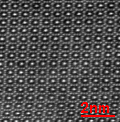
\includegraphics[width=0.7\textwidth]{img/chapitre1/figure7/drift-sc.png}
        \caption{Un exemple de défaut en haute résolution : la dérive de l'échantillon. L'échantillonnage se fait ligne par ligne. On observe que, dans ce cas, l'échantillon dérive sur la gauche, puis vers le haut. Il en résulte une déformation notable et préjudiciable du réseau atomique.
            \protect\label{fig-drift}}
    \end{marginfigure}

    \subsection{ACP et redondance spectrale}\label{sec-acp-redondance}

    Le spectre-image \gls{eels} comporte généralement une grande quantité de pixels $\gls{P}\approx 10^4$ et de canaux $\gls{M}\approx 10^3$, conduisant à un nombre de coefficients de l'ordre de $10^7$. La très grande dimension de ces données complique toute analyse directe de l'image et l'on cherche à simplifier l'étude en réduisant la taille des données tout en conservant le maximum d'information intrinsèque. Un outil fondamental permettant cela est l'\gls{acp} qui réduit la dimension des données en extrayant les composantes les plus informatives. Cette technique présentée dans cette section s'appuie sur une propriété essentielle des données \gls{eels} : la redondance spectrale.

    \paragraph{Présentation générale de l'ACP.} L'\gls{acp} est une technique utilisée en analyse multivariée qui consiste à transformer $M$ variables corrélées entre elles en autant de nouvelles variables décorrélées les unes des autres~\cite{jolliffe2002springer}. Pour cela, la transformation estime successivement les axes dans $\mathbb{R}^M$ maximisant la variance des variables projetées sur cet axe (à chaque nouvel axe estimé, sa contribution est soustraite aux données avant d'estimer l'axe suivant). Ces axes successifs sont appelés les \emph{composantes principales des données}.
    %
    Nous décrivons succinctement l'application de l'\gls{acp} à un spectre-image constituée de $P$ pixels et $M$ canaux, représenté par la matrice $\gls{Y} \in \mathbb{R}^{M\times P}$. Chaque ligne de cette matrice est une image 2D associé à un canal tandis que chaque colonne est le spectre mesuré en une position spatiale donnée.
    %
    Par simplicité de l'exposé, à l'image $\mathbf{Y}$ est associée une image centrée $\tilde{\mathbf{Y}}$, \ie\ obtenue après soustraction de la moyenne empirique des spectres, $\tilde{\mathbf{Y}}=\gls{Y}-\frac{1}{P}\sum_p\mathbf{y}_p$.
    %
    Ainsi, l'ACP transforme l'image $\tilde{\gls{Y}}$ dont les canaux sont possiblement corrélés en les données transformées $\mathbf{S}$ (aussi appelées \emph{variables de représentation}) décorrélées
    \begin{equation}\label{eq-decomposition-acp}
    \mathbf{S} = \gls{H}^T\tilde{\gls{Y}}
    \end{equation}
    où $\gls{H} = [\mathbf{h}_1,\dots,\mathbf{h}_M]$ est une matrice orthogonale de taille \taille{M}{M} contenant les composantes principales de \gls{Y}. Remarquons que l'orthogonalité de \gls{H} dans la transformation~\eqref{eq-decomposition-acp} permet de considérer l'\gls{acp} comme un changement de base dans $\mathbb{R}^M$ dont les vecteurs $\mathbf{h}_1,\dots,\mathbf{h}_M$ forment la nouvelle base. 
    %
    En pratique, la matrice $\gls{H}$ est obtenue en diagonalisant la matrice de variance-covariance $\tilde{\mathbf{C}} = \frac{1}{p-1}\tilde{\gls{Y}}\tilde{\gls{Y}}^T$. Les vecteurs propres constituent la matrice $\gls{H}$ tandis que chaque valeur propre $\gls{d}_m$ correspond à la variance de la représentation $\mathbf{s}_m$ pour une composante principale $\mathbf{h}_m$ donnée. On désigne ainsi la valeur propre $\gls{d}_m$ comme la puissance associée à la composante principale $\mathbf{h}_m$ et les colonnes de \gls{H} sont triées par puissance décroissante. 
    %
    Enfin, précisons que l'estimation des composantes principales est d'autant meilleure que la matrice de covariance est correctement estimée, \ie\ dans des régimes tels que $P\gg M$.

    \paragraph{Matrice de covariance ou matrice de corrélation ?} Dans le paragraphe précédent, la moyenne empirique $\boldsymbol\mu = [\mu_1,\dots,\mu_M]^T$ a été soustraite aux données afin d'obtenir les données centrées
    \begin{equation}
     \tilde{\mathbf{Y}} =
        \begin{pmatrix}
        y_{1,1} - \mu_1&y_{1,2} - \mu_1&\cdots&y_{1,P} - \mu_1\\
        y_{2,1} - \mu_2&y_{2,2} - \mu_2&\cdots&y_{2,P} - \mu_2\\
        \vdots&\vdots&\ddots&\vdots\\
        y_{M,1} - \mu_M&y_{M,2} - \mu_M&\cdots&y_{M,P} - \mu_M
        \end{pmatrix}.
    \end{equation}
    La matrice de covariance $\tilde{\mathbf{C}} = \frac{1}{p-1}\tilde{\gls{Y}}\tilde{\gls{Y}}^T$ est ensuite calculée afin d'extraire les composantes principales. Cette méthode a un défaut majeur : si un canal d'indice $m_0\in\llbracket 1,M\rrbracket$ correspond à un seuil d'amplitude très supérieure aux amplitudes des autres seuils, alors celui-ci va \guillemets{tirer} les résultats de l'ACP vers lui au détriment des autres caractéristiques~\cite[Section~3.3]{jolliffe2002springer}.
    %
    Dans ce genre de cas, l'alternative consiste à estimer les écarts-types empiriques $\boldsymbol\sigma=[\sigma_1,\dots,\sigma_M]^T$, puis à réduire les données centrées
    \begin{equation}
    \bar{\mathbf{Y}} =
    \begin{pmatrix}
    \frac{y_{1,1} - \mu_1}{\sigma_1}&
    \frac{y_{1,2} - \mu_1}{\sigma_1}&
    \cdots&
    \frac{y_{1,P} - \mu_1}{\sigma_1}\\
    %
    \frac{y_{2,1} - \mu_2}{\sigma_2}&
    \frac{y_{2,2} - \mu_2}{\sigma_2}&
    \cdots&
    \frac{y_{2,P} - \mu_2}{\sigma_2}\\
    %
    \vdots&\vdots&\ddots&\vdots\\
    %
    \frac{y_{M,1} - \mu_M}{\sigma_M}&
    \frac{y_{M,2} - \mu_M}{\sigma_M}&
    \cdots&
    \frac{y_{M,P} - \mu_M}{\sigma_M}
    \end{pmatrix}.
    \end{equation}
    La matrice de \emph{corrélation} $\bar{\mathbf{C}} = \frac{1}{p-1}\bar{\gls{Y}}\bar{\gls{Y}}^T$ est ensuite diagonalisée afin d'extraire les composantes principales. %
    %
    Si cette technique permet de prévenir le défaut lié à la matrice de covariance, elle présente elle-même un inconvénient puisqu'elle est plus apte à capturer des seuils apparentés au bruit.
    %
    Ces aspects sont détaillés et discutés à l'annexe~\ref{abstr-pca-corr-cov}. Dans le cadre de cette étude, la matrice de covariance sera utilisée.


    \paragraph{L'ACP en vue de réduire la dimension.} L'ACP est d'autant plus performante à réduire la dimension des données que celles-ci sont corrélées. En effet, si les observations sont fortement corrélées, on observe que les variances des variables de représentation associées aux premières composantes principales sont particulièrement élevées par rapport aux variances des variables de représentation associées aux dernières composantes principales.
    %
    Ainsi, l'on observe généralement un changement de comportement à un indice $\gls{R}\ll M$ d'autant plus faible que les données sont corrélées. \`A défaut de variation brutale de la courbe des puissances, on choisit l'indice \gls{R} tel que les \gls{R} premières composantes principales regroupent une fraction élevée de la puissance totale.
    %
    Dans ce cas, il est possible d'approcher les données \gls{Y} par une matrice $\hat{\gls{Y}}^{1:R}$ en projetant les données sur le sous-espace de dimension \gls{R} généré par les \gls{R} premières composantes principales, puis en les rétro-projetant dans $\mathbb{R}^M$. Ainsi, l'approximation à l'ordre \gls{R} s'écrit
    \begin{equation}
    \hat{\gls{Y}}^{1:R} = \gls{H}_{1:R}\gls{H}_{1:R}^T\gls{Y}
    \end{equation}
    où $\gls{H}_{1:R}$ correspond aux $R$ premières colonnes de $\gls{H}$. Cette approximation est d'autant plus fidèle que les données sont fortement corrélées, comme le montre la \cref{fig-pca-data-corr}.

    \begin{figure*}[]
        \centering
        \subfigure[\label{fig-pca-data-corr-a}$\mathrm{corr} = 0$]{
            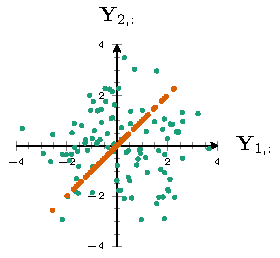
\includegraphics{img/chapitre1/figure15/pca-corr-1.pdf}}
        \subfigure[\label{fig-pca-data-corr-b}$\mathrm{corr} = 0.95$]{
            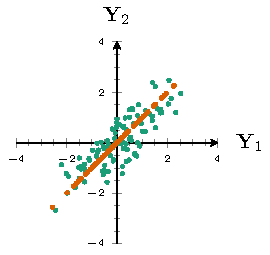
\includegraphics{img/chapitre1/figure15/pca-corr-2.pdf}}
        \subfigure[\label{fig-pca-data-corr-c}$\mathrm{corr} = 0.99$]{
            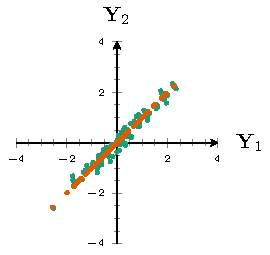
\includegraphics{img/chapitre1/figure15/pca-corr-3.pdf}}
        \caption{Trois exemples de nuages de points avec $M=2$ et $P=100$ (en vert) et leur approximation au 1er ordre (en orange). Les coefficients de corrélation valent respectivement 0, 0.95 et 0.99 pour les figures~\protect\subref{fig-pca-data-corr-a}, \protect\subref{fig-pca-data-corr-b} et \protect\subref{fig-pca-data-corr-c}. L'approximation du premier ordre est d'autant meilleure que les données sont corrélées. En particulier, ne conserver que la première composante principale est suffisant pour la figure~\protect\subref{fig-pca-data-corr-c}.
            \protect\label{fig-pca-data-corr}}
    \end{figure*}

    \paragraph{Application aux données EELS.} L’imagerie hyperspectrale est une technique combinant l’imagerie et la spectroscopie où chaque pixel de l'image est caractérisé par un spectre électromagnétique. Ces images spectroscopiques sont utilisés dans de nombreux domaines incluant la télédétection~\cite{schaepman2009earth}, la planétologie~\cite{smith1985quantitative}, le contrôle des aliments~\cite{gowen2007hyperspectral} et l'ingénierie biomédicale~\cite{akbari2010detection}. Si les spectres \gls{eels} ne sont pas de nature électromagnétiques, ils partagent néanmoins avec les images hyperspectrales un très grand nombre de propriétés et de méthodes d'analyse.
    %
    La popularité de ces techniques découle d'une propriété fondamentale des données hyperspectrales~: la redondance spectrale. En effet, les spectres issus de ces images sont connus pour être fortement corrélés spectralement~\cite{dobigeon2016linear, bioucas2012hyperspectral, dobigeon2012spectral} et le paradigme du démélange (discuté en détail à la \cref{sec-demelange}) en donne une interprétation physique. Dans ce paradigme, chaque spectre acquis est supposé être le mélange de signatures spectrales élémentaires appelés \emph{endmembers} correspondant à des éléments particuliers de la scène (\eg{} de l'eau, des bâtiments ou de la végétation en télédétection).
    %
    Tout cela permet de conclure que les spectres, loin de remplir $\mathbb{R}^M$ uniformément, évoluent dans une variété de dimension $\gls{R}\ll M$. Par défaut, cette variété n'est pas plane puisque des non-linéarités interviennent dans le mélange, causés par des phénomènes physiques au niveau local\footnote{Voir par exemple~\cite{dobigeon2014nonlinear} pour une discussion de ces phénomènes dans le cas de l'imagerie hyperspectrale.}. Néanmoins, une approximation linéaire peut être réalisée afin d'estimer le sous-espace de dimension réduite appelé \emph{sous-espace signal}, possiblement à l'aide d'une \gls{acp}. L'identification de ce sous-espace permet d'obtenir des variables de représentation de dimension réduite pourtant très précises, ouvrant la voie à un gain considérable en temps de calcul, en complexité et en stockage de donnée pour une qualité d'image équivalente. Comme expliqué plus haut, l'\gls{acp} réduit d'autant la dimension du spectre-image (ou encore \gls{R} est d'autant plus faible) que les données sont corrélées \ie{} que peu d'éléments élémentaires sont présent dans la scène. La \cref{fig-ACP} montre les composantes principales d'un spectre-image réel. L'évolution des puissances issues de l'\gls{acp} affichées à la \cref{fig-sub-pca-eigs} nous permet de déterminer trois comportements\footnote{Il faut noter que les puissances ont été corrigées afin de compenser l'erreur d'estimation dû au faible nombre d'observations (le nombre de pixels est du même ordre de grandeur que le nombre de canaux), comme expliqué à la \cref{subsec-3s-acp}.}.
    \begin{normalfigure*}[htbp]
        \centering
        \subfigure[Evolution des valeurs propres associées à l'\gls{acp}]{
            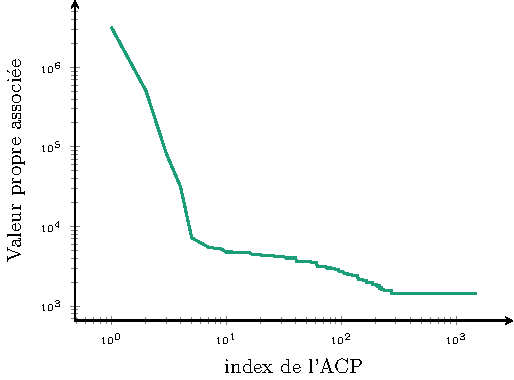
\includegraphics[]{img/chapitre1/figure9/PCA_eigs.pdf}
            \label{fig-sub-pca-eigs}}
        \\
        \subfigure[Variable de repr. \num\ 1]{\label{fig-sub-pca-comp1}
            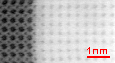
\includegraphics[width=0.28\textwidth]{img/chapitre1/figure9/PCA_map_0-sc.png}}\vspace{20pt}
        \subfigure[Variable de repr. \num\ 2]{\label{fig-sub-pca-comp2}
            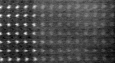
\includegraphics[width=0.28\textwidth]{img/chapitre1/figure9/PCA_map_1.png}}\vspace{20pt}
        \subfigure[Variable de repr. \num\ 3]{\label{fig-sub-pca-comp3}
            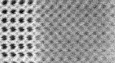
\includegraphics[width=0.28\textwidth]{img/chapitre1/figure9/PCA_map_2.png}}\\
        \subfigure[Variable de repr. \num\ 4]{\label{fig-sub-pca-comp4}
            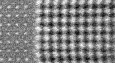
\includegraphics[width=0.28\textwidth]{img/chapitre1/figure9/PCA_map_3.png}}\vspace{20pt}
        \subfigure[Variable de repr. \num\ 5]{\label{fig-sub-pca-comp5}
            
\includegraphics[width=0.28\textwidth]{img/chapitre1/figure9/PCA_map_4.png}}\vspace{20pt}
        \subfigure[Variable de repr. \num\ 6]{\label{fig-sub-pca-comp6}
            
\includegraphics[width=0.28\textwidth]{img/chapitre1/figure9/PCA_map_5.png}
        }\\
        %
        \def\comp{mean}
        \subfigure[Spectre moyen]{
            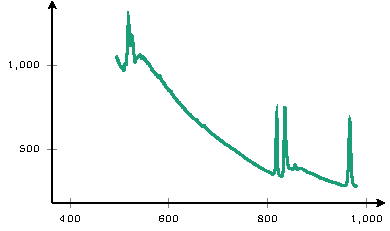
\includegraphics[]{img/chapitre1/figure9/PCA_spectra_1.pdf}
            \label{fig-sub-pca-mean}}%
        %
        \def\comp{comp0}%
        \subfigure[Première composante]{
            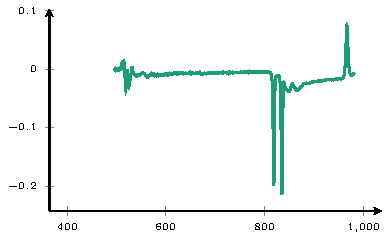
\includegraphics[]{img/chapitre1/figure9/PCA_spectra_2.pdf}
            \label{fig-sub-pca-spectrum-0}}
        %
        \caption{\gls{acp} de données \gls{eels}. La figure~\subref{fig-sub-pca-eigs} représente l'évolution des valeurs propres associées à l'\gls{acp}. On observe, entre autres, que seules les 5 premières composantes sont vraiment significatives. Les figures \subref{fig-sub-pca-comp1} à \subref{fig-sub-pca-comp6} représentent les variables de représentation associées aux composantes principales les plus puissantes. Le spectre moyen donné à la figure~\subref{fig-sub-pca-mean} est soustrait aux données avant d'appliquer l'\gls{acp}. Il en résulte que les spectres associés aux composantes principales sont des variations par rapport à ce spectre moyen, ce qui explique que la première composante affichée à la figure~\subref{fig-sub-pca-spectrum-0} soit parfois à valeurs négatives.
            \protect\label{fig-ACP}}
    \end{normalfigure*}    
    \begin{itemize}
        \item Les premières composantes de puissance très élevées correspondent à des éléments chimiques présents en forte quantité dont les projections associées (\cf{} \crefrange{fig-sub-pca-comp1}{fig-sub-pca-comp4}) renferment beaucoup d'information spatiale et peu de bruit. Le spectre associé à la première composante est lui-même très peu bruité (\cf{} \cref{fig-sub-pca-spectrum-0}).
        \item Un ensemble de composantes principales situées entre les indices 5 et 300 se démarque encore par sa puissance, bien que moins important que les premières composantes. L'évolution de leur puissance est également moins rapide. Il s'agit généralement de composants très localisés spatialement ou issus de mélanges non-linéaires. Certaines informations spatiales peuvent être encore discernées chez les projections associées aux composantes les plus puissantes, comme à la \cref{fig-sub-pca-comp5}.
        \item Les dernières composantes présentent enfin une puissance constante correspondant à la puissance estimée du bruit. Plus aucune information n'est visible ni dans le spectre associé ni dans la projection correspondante.
    \end{itemize}
    Cette observation permet généralement le débruitage des données en supprimant les composantes principales associées au bruit, comme décrit à la \cref{sec-ech-sensibles}. Malheureusement, le choix du seuil \gls{R} correspondant à la dimension du sous-espace estimé n'est pas trivial. Deux solutions seront cependant proposées: l'une basée sur l'évolution des valeurs propres à la \cref{subsec-3s-acp}, l'autre analysant le contenu spatial des images issues des projections sur les composantes principales à l'annexe~\ref{sec-spim-creation-hr}

    

    %
    \section{Cartographie par séparation de composantes spectrales}\label{sec-exploitation-eels}

    Le problème généralement rencontré lors de l'exploitation des données \gls{eels} consiste à localiser et à cartographier un ensemble de composés chimiques élémentaires présents dans l'échantillon~\cite{colliex2012stem, pennycook2011seeing, dobigeon2012spectral}.
    %
    Pour cela, nous pouvons exploiter l'information spectrale contenue aux abords du seuil associé à l'élément étudié. En effet, plus il est abondant en une position spatiale, plus l'amplitude du seuil associé est grande. En couplant l'information obtenue en chaque position, une image appelée \emph{carte d'abondance} renseignant sur sa répartition spatiale peut être générée. 
    %
    Ce problème est plus largement rencontré en imagerie hyperspectrale, comme en télédétection afin de cartographier des constituants élémentaires au sein d'une scène~\cite{lelong1998hyperspectral} (\eg{} eau, bâtiments, etc).
    %
    La technique historique classiquement utilisée en imagerie \gls{eels} analyse de manière supervisée les spectres pris indépendamment afin de quantifier un élément particulier.
    %
    A l'inverse, des approches plus récentes analysent le spectre-image dans son entièreté de manière non-supervisée afin de cartographier l'ensemble des composants d'intérêt. 
    %
    La cartographie de composés chimiques ne constitue pas le c\oe{}ur de la thèse, mais elle peut être utilisée pour évaluer la qualité de la reconstruction, comme à la section~\ref{sec-lr-demelange-res}.


    \subsection{Quantification par ajustement d'exponentielle}
    
    Comme expliqué à la \cref{sec-prop-eels}, un spectre \gls{eels} contient la contribution de plusieurs seuils successifs et d'un fond continu. Pour pallier ce problème, le fond décroissant et la rémanence des seuils précédents devront être soustraits avant d'intégrer le seuil d'intérêt. Pour illustrer cette méthode, considérons le spectre affiché à la \cref{fig-carto-separation-a}, correspondant à une position spatiale donnée. Une zone de régression est choisie en amont du seuil (tout en restant proche du seuil) et une régression exponentielle de la forme $y=Ax^{-r}$ est effectuée (\cf{}~\cite[Section~4.4]{egerton2011electron} pour plus de détails). La courbe estimée est alors soustraite pour obtenir un spectre corrigé propre à ce seuil, \ie{}, le seuil étudié n'est plus influencé par le fond continu. L'abondance du composé pour cette position spatiale est ensuite calculée en sommant le spectre dans une zone centrée sur le seuil d'intérêt. En effectuant cette opération pour toutes les positions spatiales, nous pouvons reconstituer la carte d'abondance de la \cref{fig-carto-separation-b}. \`A noter que les paramètres de la régression dépendent de la position spatiale.

    Afin d'effectuer la cartographie de plusieurs composantes présentes dans l'échantillon, l'expérimentateur doit alors exécuter cette opération pour tous les seuils présents dans le spectre. Cette technique est simple et une implémentation automatique est facile à mettre en \oe{}uvre dès lors que les zones de régression et d'intégration ont été définies.
    
    \begin{figure*}[t]
        \centering
        \subfigure[\label{fig-carto-separation-a}]{
            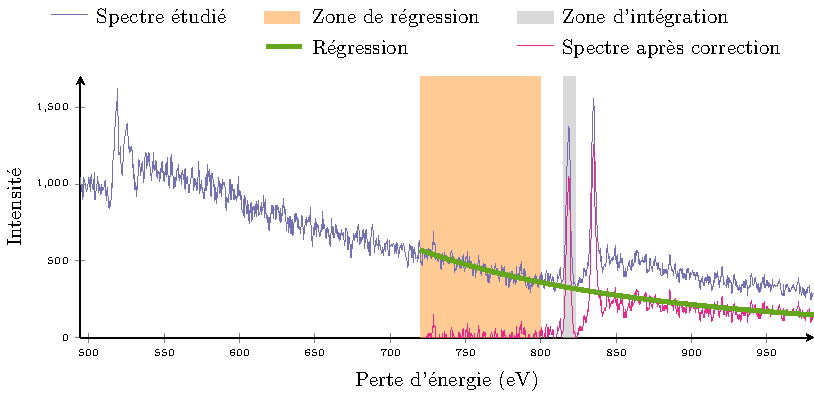
\includegraphics[]{img/chapitre1/figure11/separation.pdf}}\hspace{1em}
        \subfigure[\label{fig-carto-separation-b}]{
            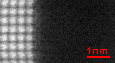
\includegraphics[width=5cm]{img/chapitre1/figure11/regression-sc.png}}
        \caption{Illustration de la méthode de cartographie par ajustement d'exponentielles spectrales. \protect\subref{fig-carto-separation-a} Régression pour une position particulière. Une régression exponentielle est effectuée sur la zone de régression, puis est soustraite au spectre pour obtenir le spectre corrigé. L'abondance est finalement calculée en intégrant le spectre autour du pic d'intérêt. \protect\subref{fig-carto-separation-b} Résultat en effectuant cette action sur tous les pixels (l'élément cartographié est $\mathrm{La-M}_{4, 5}$). A noter que les paramètres de la régression dépendent de la position spatiale.
            \protect\label{fig-carto-separation}}
    \end{figure*}
    
    Cependant, cette technique ne permet que la \emph{quantification} de l'élément à une constante près quel que soit son environnement\,; elle ne permet entre autres pas d'obtenir des proportions contrairement au démélange discuté à la section suivante. Or, la structure fine, \ie\ la forme du seuil, renseigne sur l'état du composé étudié et la technique ci-dessus ne fait aucune distinction lors de la quantification. Par exemple, les travaux menés dans~\cite{dobigeon2012spectral} s'intéressent à l'état d'oxydation du bore et tentent de cartographier deux états distincts, la forme oxydée B\textsubscript{2}O\textsubscript{3} et la forme azotée BN. Dans ce cas, la technique proposée ne fait pas cette distinction.
    %
    Pour résoudre cette impasse, des techniques de cartographie non-supervisée ont été proposées ces dernières décennies afin de ne pas considérer le pic uniquement, mais l'ensemble du spectre.

    

    \subsection{Techniques de cartographie non-supervisée}\label{sec-demelange}
    
    \paragraph{Approches par ACP et ACI.} La redondance spectrale présentée à la section précédente suggère que les spectres acquis soient le résultat d'un mélange de $N_c$ spectres élémentaires $\mathbf{m}_1,\dots,\mathbf{m}_{N_c}$ appelés \emph{endmembers}, correspondant aux signatures associées aux composés caractéristiques présents dans l'échantillon.
    %    
    Estimer les signatures $\mathbf{m}_k$ s'apparente à de la séparation aveugle de sources et les premières techniques non-supervisée proposées l'ont considérée d'un point de vue statistique en usant des techniques d'analyse multivariée. Dans cette perspective, l'\gls{acp} a été utilisée afin d'extraire les signatures de spectre-images \gls{eels} dans~\cite{bonnet1999extracting, bosman2006mapping, trebbia1990eels}, mais cette méthode renvoie des spectres difficiles à interpréter physiquement, à cause notamment de la contrainte d'orthogonalité inhérente à l'\gls{acp} imposée aux endmembers. L'\gls{aci} a été envisagée comme alternative afin d'analyser les données hyperspectrales issues de la télédétection~\cite{bayliss1998analyzing, chen1999independent} ou de l'imagerie \gls{stem}-\gls{eels}~\cite{delapena2011mapping, bonnet2005independent, bosman2006mapping}. Malheureusement, l'\gls{aci} repose sur l'hypothèse que les signatures spectrales comme leur abondance soient indépendantes, ce qui n'est pas le cas puisque si un élément est fortement présent, les autres le seront généralement moins. Cela compromet l'utilisation de l'\gls{aci} en démélange hyperspectral, d'autant que ni l'\gls{acp}, ni l'\gls{aci} ne permettent de contraindre l'abondance à être positive et leurs résultats demeurent en général difficiles à interpréter d'un point de vue physique. Toutefois, l'ACI peut donner des résultats intéressants et rapides pour certains jeux de données et cela peut être un point de départ dans l'analyse de l'image.
    
    \paragraph{Approches par démélange.} Comme expliqué précédemment, les spectres acquis sont supposés être le résultat d'un mélange de $N_c$ spectres élémentaires\,; une hypothèse de mélange linéaire est souvent réalisée afin de simplifier l'interprétation et la résolution du problème associé. %
    %
    Notons que ce modèle permet également de générer des spectres-images EELS réalistes, à partir de spectres caractéristiques réels et de carte d'abondances réalistes. Ce procédé a notamment été mis en oeuvre à la section~\ref{sec-synth-data-lr}.
    %
    Dans ce cas, le modèle s'écrit~\cite{dobigeon2016linear}
    \begin{align}
    &\gls{Y} \approx \mathbf{M}\mathbf{A}\\
    \text{tel que}\quad &\mathbf{A} \geq 0\qquad \mathbf{M} \geq 0\label{eq-positivity}\\
    &\sum_k a_{kp} = 1 \quad \forall p\in\llbracket 1 , P \rrbracket \label{eq-sum-to-one}
    \end{align}
    où $\mathbf{M}=[\mathbf{m}_1,\dots,\mathbf{m}_{N_c}]$ de taille $M\times N_c$ est la matrice contenant les signatures spectrales et où $\mathbf{A}$ est la matrice d'abondance de taille $N_c\times P$. Chaque ligne $\mathbf{A}_{k,:}$ est une image représentant la proportion de l'endmember $\mathbf{m}_k$ au sein de l'échantillon, il s'agit de la carte d'abondance. Deux hypothèses portant sur $\mathbf{A}$ sont réalisées : l'hypothèse de positivité à l'équation~\eqref{eq-positivity} et l'hypothèse de somme à un à l'équation~\eqref{eq-sum-to-one}.
    \begin{description}
        \item[Positivité] L'abondance de l'élément ne peut être négative puisqu'il s'agit d'une proportion. Et puisque le spectre est positif, les entrées de $\mathbf{A}$ et de $\mathbf{M}$ sont donc positives.
        \item[Somme à un] La somme des abondances vaut un pour toute position spatiale. Cette hypothèse traduit le fait que les éléments de $\mathbf{A}$ soient des proportions. Cependant, pour que l'on puisse comparer les proportions d'un pixel à l'autre, il est nécessaire que la quantité de matière traversée par le faisceau soit la même sur l'ensemble de l'échantillon, sans quoi deux proportions identiques ne traduiraient pas une quantité égale de l'élément.
    \end{description}
    Une représentation géométrique du mélange linéaire est donné à la \cref{fig-melange-lineaire} pour $M=3$ et $N_c=3$. Les coordonnées des trois endmembers $\mathbf{m}_1,\mathbf{m}_2,\mathbf{m}_3$ sont représentés dans $\mathbb{R}^3$ et puisque la contrainte de somme à un est utilisée ici, l'ensemble des spectres obtenus par mélange linéaire se situent dans le plan de dimension $M-1=2$ généré par ces trois vecteurs (à condition qu'ils soient linéairement indépendants). Enfin, l'hypothèse de positivité contraint l'ensemble des spectres de \gls{Y} à évoluer dans le simplexe formé par $\mathbf{m}_1$, $\mathbf{m}_2$ et $\mathbf{m}_3$.
    \begin{figure}
        \centering
        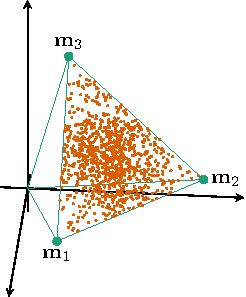
\includegraphics[]{img/chapitre1/figure17/melange_lineaire.pdf}
        \caption{Une représentation géométrique du modèle de mélange linéaire pour $M=3$ et $N_c=3$. Les spectres élémentaires sont notés $\mathbf{m}_1$, $\mathbf{m}_2$ et $\mathbf{m}_3$. La contrainte de somme à un contraint les spectres constitutifs de \gls{Y} (en orange) à évoluer dans le plan formé par ces trois vecteurs tandis que la contrainte de positivité les contraint à demeurer dans le simplexe formé par les endmembers.
            \protect\label{fig-melange-lineaire}}
    \end{figure}
    Maintenant que le modèle est posé, le problème consiste à estimer conjointement les spectres élémentaires $(\mathbf{m}_k)_{k=1,\dots,N_c}$ ainsi que les cartes d'abondance associées. Ce problème est appelé \emph{démélange hyperspectral}~\cite{bioucas2012hyperspectral, dobigeon2016linear} ou \emph{unmixing} et s'apparente à un problème de séparation aveugle de source~\cite{comon2010handbook}. Il requiert la connaissance du nombre de composantes $N_c$.
    %
    Une technique de démélange non-supervisée a pour but d'estimer les endmembers, ou de manière géométrique le simplexe dans lequel évoluent les spectres acquis et dont les endmembers constituent les sommets, et la matrice d'abondance associée\footnote{Le nombre d'endmember est lui-aussi inconnu dans la plupart des situations, mais il peut être estimé par une autre méthode a priori.}. Souvent, ce problème d'estimation est généralement non-convexe et on lui préfère une résolution sous-optimale en deux temps. D'abord, les signatures élémentaires sont déterminées à l'aide d'un algorithme d'extraction d'endmember, puis la matrice d'abondance est déterminée. Néanmoins, des méthodes bayésiennes permettent une estimation conjointe des endmembers et de des abondances basées sur un modèle statistique.

    \paragraph{Estimation des endmembers.} Les premières méthodes d'extraction d'endmember utilisées furent l'ACP et l'ACI avec les inconvénients relevés plus haut.
    % 
    Une autre approche du problème consiste à user de l'interprétation géométrique réalisée plus haut afin d'estimer les endmembers $\mathbf{m}_k$. Dans l'hypothèse où les composantes pures sont présentes dans l'échantillon, des techniques efficaces et rapides permettent de déterminer les spectres acquis correspondant aux endmembers. Par exemple, \gls{vca}~\cite{nascimento2005vertex} projette itérativement les données sur un axe orthogonal au sous-espace généré par les endmembers déjà déterminés. Le nouvel endmember correspond au point extrême de la projection et l'algorithme est itéré jusqu'à obtenir toutes les composantes. Néanmoins, l'hypothèse de pixels purs est généralement trop forte. En microscopie \gls{stem}-\gls{eels}, par exemple, à cause d'une résolution insuffisante ou d'une épaisseur d'échantillon permettant la superposition d'éléments différents, on n'acquiert pas de spectre pur. Pour relâcher cette contrainte, les techniques par minimisation de volume estiment la matrice $\mathbf{M}$ de sorte que le simplexe généré par les endmembers $\mathbf{m}_k$ soit de volume minimal tout en contenant l'ensemble des spectres acquis. Ce problème devient plus difficile à résoudre puisqu'il est non-convexe, c'est pourquoi il est initialisé à l'aide d'une autre technique comme \gls{vca}. L'algorithme \gls{sisal}~\cite{bioucas2009variable} implémente une version plus robuste en autorisant la violation de la contrainte de positivité, c'est pourquoi certains spectres estimés par SISAL peuvent être négatifs, mais cette violation est contrainte à l'aide de la fonction hinge $h$ ($h(x) = 0$ si $x \geq 0$ et $h(x)=-x$ si $x<0$). Les techniques par approche géométrique sont rapides et efficaces si l'image présente des pixels purs, autrement, leurs performances sont réduites et des techniques statistiques sont à préférer.
    
    \paragraph{Estimation des abondances.} Une fois l'extraction des endmembers réalisée, on doit estimer les abondances.  Cela consiste à déterminer le sous-ensemble optimal de signatures spectrales ainsi que les proportions associées pouvant décrire chaque pixel mélangé de l'échantillon. En pratique, il s'agit d'une régression parcimonieuse linéaire faisant appel à des régularisations parcimonieuses telles que décrites à la \cref{sec-MC-regul}, puisque le nombre de signatures spectrales utilisées pour décrire chaque pixel est supposé être faible devant $N_c$. Un représentant de cette famille de méthodes est \gls{sunsal}~\cite{bioucas2010alternating} qui propose de contraindre la parcimonie des abondances à l'aide d'une norme $\ell_1$ et de résoudre le problème d'optimisation par l'algorithme \gls{admm}~\cite{eckstein1992douglas, combettes2011proximal}.
    
    \paragraph{Estimation conjointe par méthode bayésienne.} D'autres techniques statistiques plus performantes ont également été étudiées, comme les approches bayésiennes qui résolvent les inconvénients de l'ACP et de l'ACI en introduisant des informations a priori, contraignant par là même les solutions à avoir un sens physique. Ces méthodes permettent l'estimation conjointe des endmembers et des abondances. L'algorithme \textit{bayesian linear unmixing} (BLU)~\cite{dobigeon2009joint} qui en est un exemple a été appliqué avec succès en imagerie \gls{stem}-\gls{eels}~\cite{dobigeon2012spectral}.
    
    
    %
    \section{L'acquisition d'échantillons sensibles : problématiques et stratégies}\label{sec-ech-sensibles}

    \paragraph{Problématique des échantillons sensibles.} Une problématique récurrente en microscopie est la détection de structures fines dont le seuil associé est de faible amplitude. Dans une telle situation, le \gls{snr} du spectre-image acquis doit être supérieur à un \gls{snr} minimum, nécessaire à la détection précise des structures fines. A cette fin, l'expérimentateur doit augmenter la dose totale d'électrons délivrée à chaque position de l'échantillon. Pour cela, il peut agir sur l'intensité du faisceau ou sur la durée d'exposition par position spatiale (appelé \emph{dwell time}). Quelle que soit l'approche, augmenter la dose totale accroît la détérioration subie par l'échantillon~\cite{egerton2004radiation}. Cela est particulièrement problématique pour les échantillons sensibles tels que les tissus biologiques. 
    %
    Il en résulte un compromis entre une qualité d'image satisfaisante et la préservation de l'échantillon d'étude. Pour illustrer cela, un exemple d'échantillon détérioré par une concentration trop importante d'énergie est donné à la \cref{fig-echantillon-deteriore}. Dès lors, des stratégies sont nécessaires afin d'améliorer la qualité du spectre-image (\ie{}, son \gls{snr}) sans augmenter la quantité d'énergie délivrée à l'échantillon.

    \begin{figure}[t]
        \centering
        \subfigure[\label{fig-echantillon-deteriore-a}]{%
            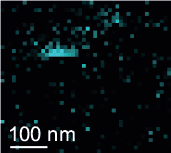
\includegraphics[width=0.3\textwidth]{img/chapitre1/figure12/sequentialScan.png}}\hspace{1em}
        \subfigure[\label{fig-echantillon-deteriore-b}]{%
            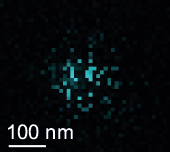
\includegraphics[width=0.3\textwidth]{img/chapitre1/figure12/randomScan.png}}
        \caption{\protect\subref{fig-echantillon-deteriore-a} Exemple d'échantillon détérioré par un faisceau trop énergétique. L'acquisition est réalisée ligne par ligne en commençant au pixel supérieur gauche. \`A un certain stade de l'acquisition, une structure apparaît puis disparaît soudainement. En effet, la structure a été détruite suite à une trop grande accumulation d'énergie, l'acquisition conventionnelle illuminant les positions successives. \protect\subref{fig-echantillon-deteriore-b} Acquisition d'une structure semblable avec un parcours aléatoire et la même énergie par pixel. La structure est elle-aussi détériorée, mais l'échantillonnage aléatoire permet de visualiser la particule avant sa disparition.
            \protect\label{fig-echantillon-deteriore}}
    \end{figure}

    \paragraph{Acquisition ligne par ligne v.s. aléatoire.} Une première solution pour réduire la détérioration de l'échantillon à énergie fixée consiste à échantillonner de manière aléatoire uniforme. En effet, l'acquisition ligne par ligne est très simple à implémenter, mais cette modalité détériore particulièrement l'échantillon puisqu'elle accumule des doses d'énergie sur des pixels voisins. Pour pallier ce problème, des travaux récents ont mis au point un obturateur coupant le faisceau au cours de l'acquisition standard~\cite{beche2016development}, permettant de limiter l'accumulation de charges au niveau local, au prix d'un sous-échantillonnage spatial. 
    %
    Afin d'échantillonner l'ensemble des pixels tout en protégeant l'échantillon, un module de balayage novateur basé sur FPGA a été mis au point au LPS~\cite{tararan2016random, zobelli2019spatial, tence2019following} dont le fonctionnement est décrit sur la figure~\ref{fig-random-scan}. Une de ses caractéristiques principales est de rendre le chemin d'acquisition hautement paramétrable où l'ensemble des positions spatiales sont stockées dans une table. L'ordre des pixels est mélangé aléatoirement lors d'une phase initiale, puis ce chemin aléatoire est chargé. 
    %
    Pour chaque nouvelle position à visiter, le module pilote des bobines magnétiques afin de positionner le faisceau sur l'échantillon tandis que l'acquisition du signal est désactivée à l'aide d'un obturateur de faisceau électrostatique. Une fois la position désirée atteinte, le faisceau illumine l’échantillon uniquement pendant le temps requis pour l’acquisition du signal, temps durant lequel la caméra est en mode d’exposition. Enfin, le faisceau est coupé et déplacé vers la position suivante.
    \begin{figure*}[t]
        \centering
        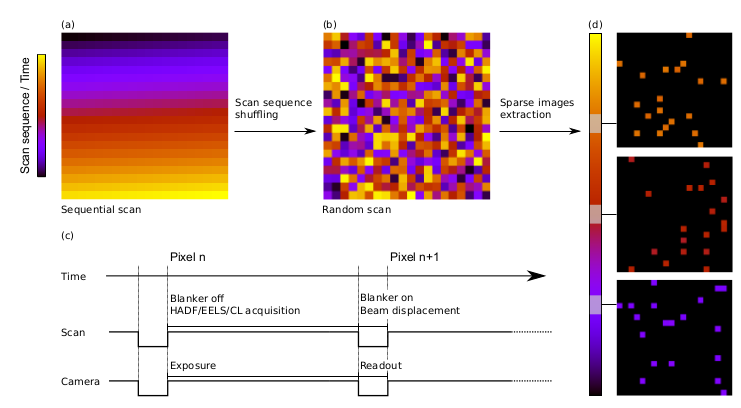
\includegraphics[width=\textwidth]{img/chapitre1/figure18/random-scan-2}
        \caption{\protect\label{fig-random-scan}Principe de l'acquisition ligne par ligne standard (a) et la séquence d'échantillonnage aléatoire (b). L'échelle de couleur représente l'ordre d'acquisition des pixels. (c) Représentation schématique de la synchronisation entre illumination, déplacement du faisceau, obstruction du faisceau, exposition et mesure. (d) Extraction d'images aléatoires partielles à certaines trames temporelles. La figure est issue de~\cite{zobelli2019spatial}.}
    \end{figure*}
    Cette technique d'acquisition permet de répartir la dose d'électrons sur l'ensemble de l'échantillon. Cela est mis en évidence à la \cref{fig-echantillon-deteriore-b} puisque la structure spatiale est totalement visible pour une acquisition aléatoire tandis que l'échantillonnage ligne par ligne  détruit prématurément la structure, comme le montre la \cref{fig-echantillon-deteriore-a}. Cette technique permet donc d'augmenter l'énergie délivrée à l'échantillon pour une détérioration égale, et donc d'améliorer la qualité de l'image.
    
    
    \paragraph{Correction de la dérive de l'échantillon.} Comme expliqué à la \cref{sec-prop-eels}, l'échantillon n'est pas nécessairement stable au cours de l'acquisition puisque des gradients de température et des mouvements d'air le font dériver. Dans le cas d'une acquisition ligne par ligne, cela se manifeste par une déformation du réseau atomique, comme le montre la \cref{fig-drift}. Dans le cas d'un échantillonnage aléatoire, cela détériore grandement la résolution spatiale, particulièrement pour les échantillons à échelle atomique. 
    %
    En pratique, la dérive est limitée en laissant l'échantillon se stabiliser après insertion dans le microscope et en s'assurant que l'acquisition soit suffisamment rapide.
    %
    Pour corriger cela, une méthode consiste à extraire $K<P$ sous-acquisitions partielles de l'acquisition aléatoire complète. Chacune de ces acquisitions partielles est alors complétée indépendamment à l'aide d'une méthode de reconstruction (cf \cref{ch-chapter_2}) et le mouvement de l'échantillon est estimé. Les échantillons associés à chaque sous-acquisition sont alors recalés pour compenser la dérive. Cette méthode est appelée \emph{multi-trame} et a été implémentée avec succès en imagerie \gls{haadf} et \gls{eels}~\cite{zobelli2019spatial}. Cette méthode améliore sensiblement la qualité de l'image, mais reste encore très peu utilisée car lourde d'un point de vue expérimental. Enfin, dans le cas d'un échantillonnage ligne par ligne où l'échantillon dérive uniformément, il est également possible de corriger le défaut par déformation géométrique du réseau.

    \paragraph{Débruitage en post-traitement.} L'approche la plus simple pour limiter la détérioration de l'échantillon consiste à réduire la dose d'électrons et à débruiter les données en post-traitement. 
    %
    Pour cela, la technique la plus couramment utilisée pour de nombreuses données spectroscopiques revient à appliquer l'\gls{acp} aux données pour ne conserver que les composantes les plus puissantes, comme cela a été fait pour réduire le bruit spectral en imagerie à échelle atomique~\cite{bosman2007two,dudeck2012quantitative}, par exemple. Cette technique rapide et simple ne permet toutefois pas d'améliorer la qualité spatiale de l'image. D'autre part, certaines études ont mis en évidence des artefacts introduits par l'\gls{acp}, comme un biais présent dans le spectre reconstruit~\cite{lichtert2013statistical, spiegelberg2017can} ou encore l'ajout de structures initialement absentes \cite{mevenkamp2017mm}.
    %
    C'est pourquoi des techniques de débruitage par patch plus récentes et plus efficaces (\cf{} \cref{sec-art-patch}) ont été appliquées afin d'accroître le \gls{snr} du spectre-image tout en limitant les distorsions. Contrairement à l'ACP, celles-ci permettent de débruiter tant spatialement que spectralement. En particulier, des techniques non-locales comme Non-Local Means~\cite{mevenkamp2017mm, mevenkamp2020multimodal} et des approches par \gls{ad} avec apprentissage~\cite{trampert2018ultramicroscopy} ont été appliquées respectivement à des données \gls{eels} et  \gls{sem}. De même, un algorithme non-local appelé Local Low Rank (LLR)~\cite{spiegelberg2018local} a été proposé et appliqué avec succès à des images 2D \gls{haadf} et à des données 3D réalisées après concaténation de cartes d'abondance obtenues par imagerie \gls{stem}-\gls{eels}.
    %
    Cependant, cette façon de préserver l'échantillon pourrait ne pas suffire si la dose maximale autorisée est trop faible. En effet, l'image serait trop dégradée pour être efficacement débruitée et les structures fines pourraient ne plus être détectées. 
    
    
    \section{Positionnement de la thèse}\label{sec-positionnement-these}

    L'équipe STEM du \gls{lps} a très tôt étudié l'ensemble des stratégies présentée dans la section précédente en vue de prévenir la destruction d'échantillons sensibles. Plus précisément, cela a été motivé par l'implémentation du module de balayage décris précédemment afin de contrôler le chemin d'acquisition. Ce système est actuellement installé sur deux microscopes \gls{stem} :
    \begin{itemize}
        \item un VG-HB501 avec un pouvoir séparateur de l’ordre du nm (\cf{} \cref{fig-LPS-micro-a}),
        \item un Nion UltraSTEM 200 équipé d’un correcteur d’aberrations sphériques qui permet d’atteindre un pouvoir séparateur de l’ordre de 0,1 nm (\cf{} \cref{fig-LPS-micro-b}).
    \end{itemize}
    %
    \begin{figure*}
        \centering  % 0.8, 0.5
        \subfigure[\label{fig-LPS-micro-a}]{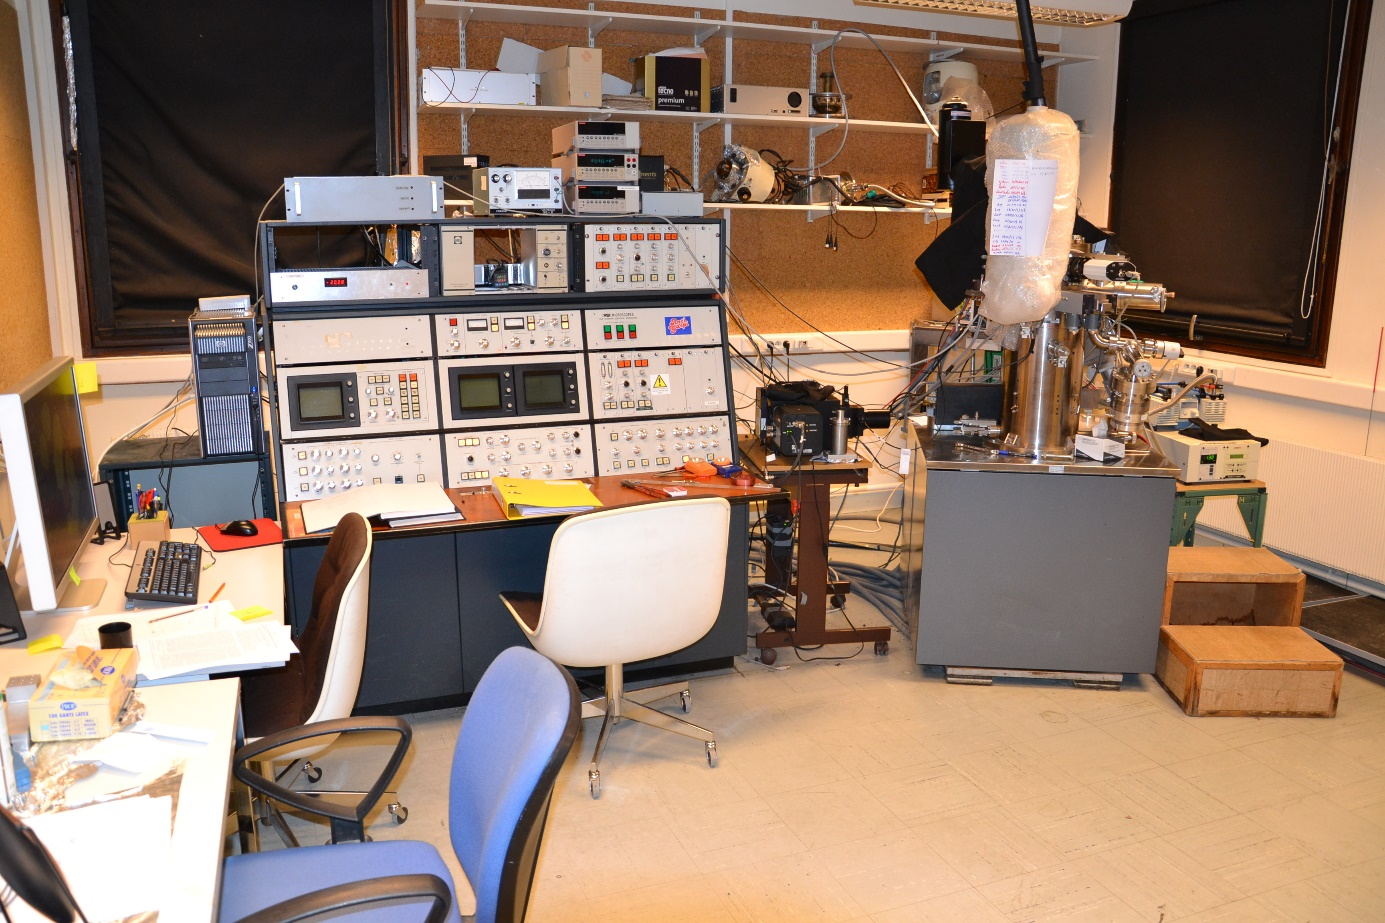
\includegraphics[width=0.5\textwidth]{img/chapitre1/figure13/VG.jpg}}
        \hspace{1em}
        \subfigure[\label{fig-LPS-micro-b}]{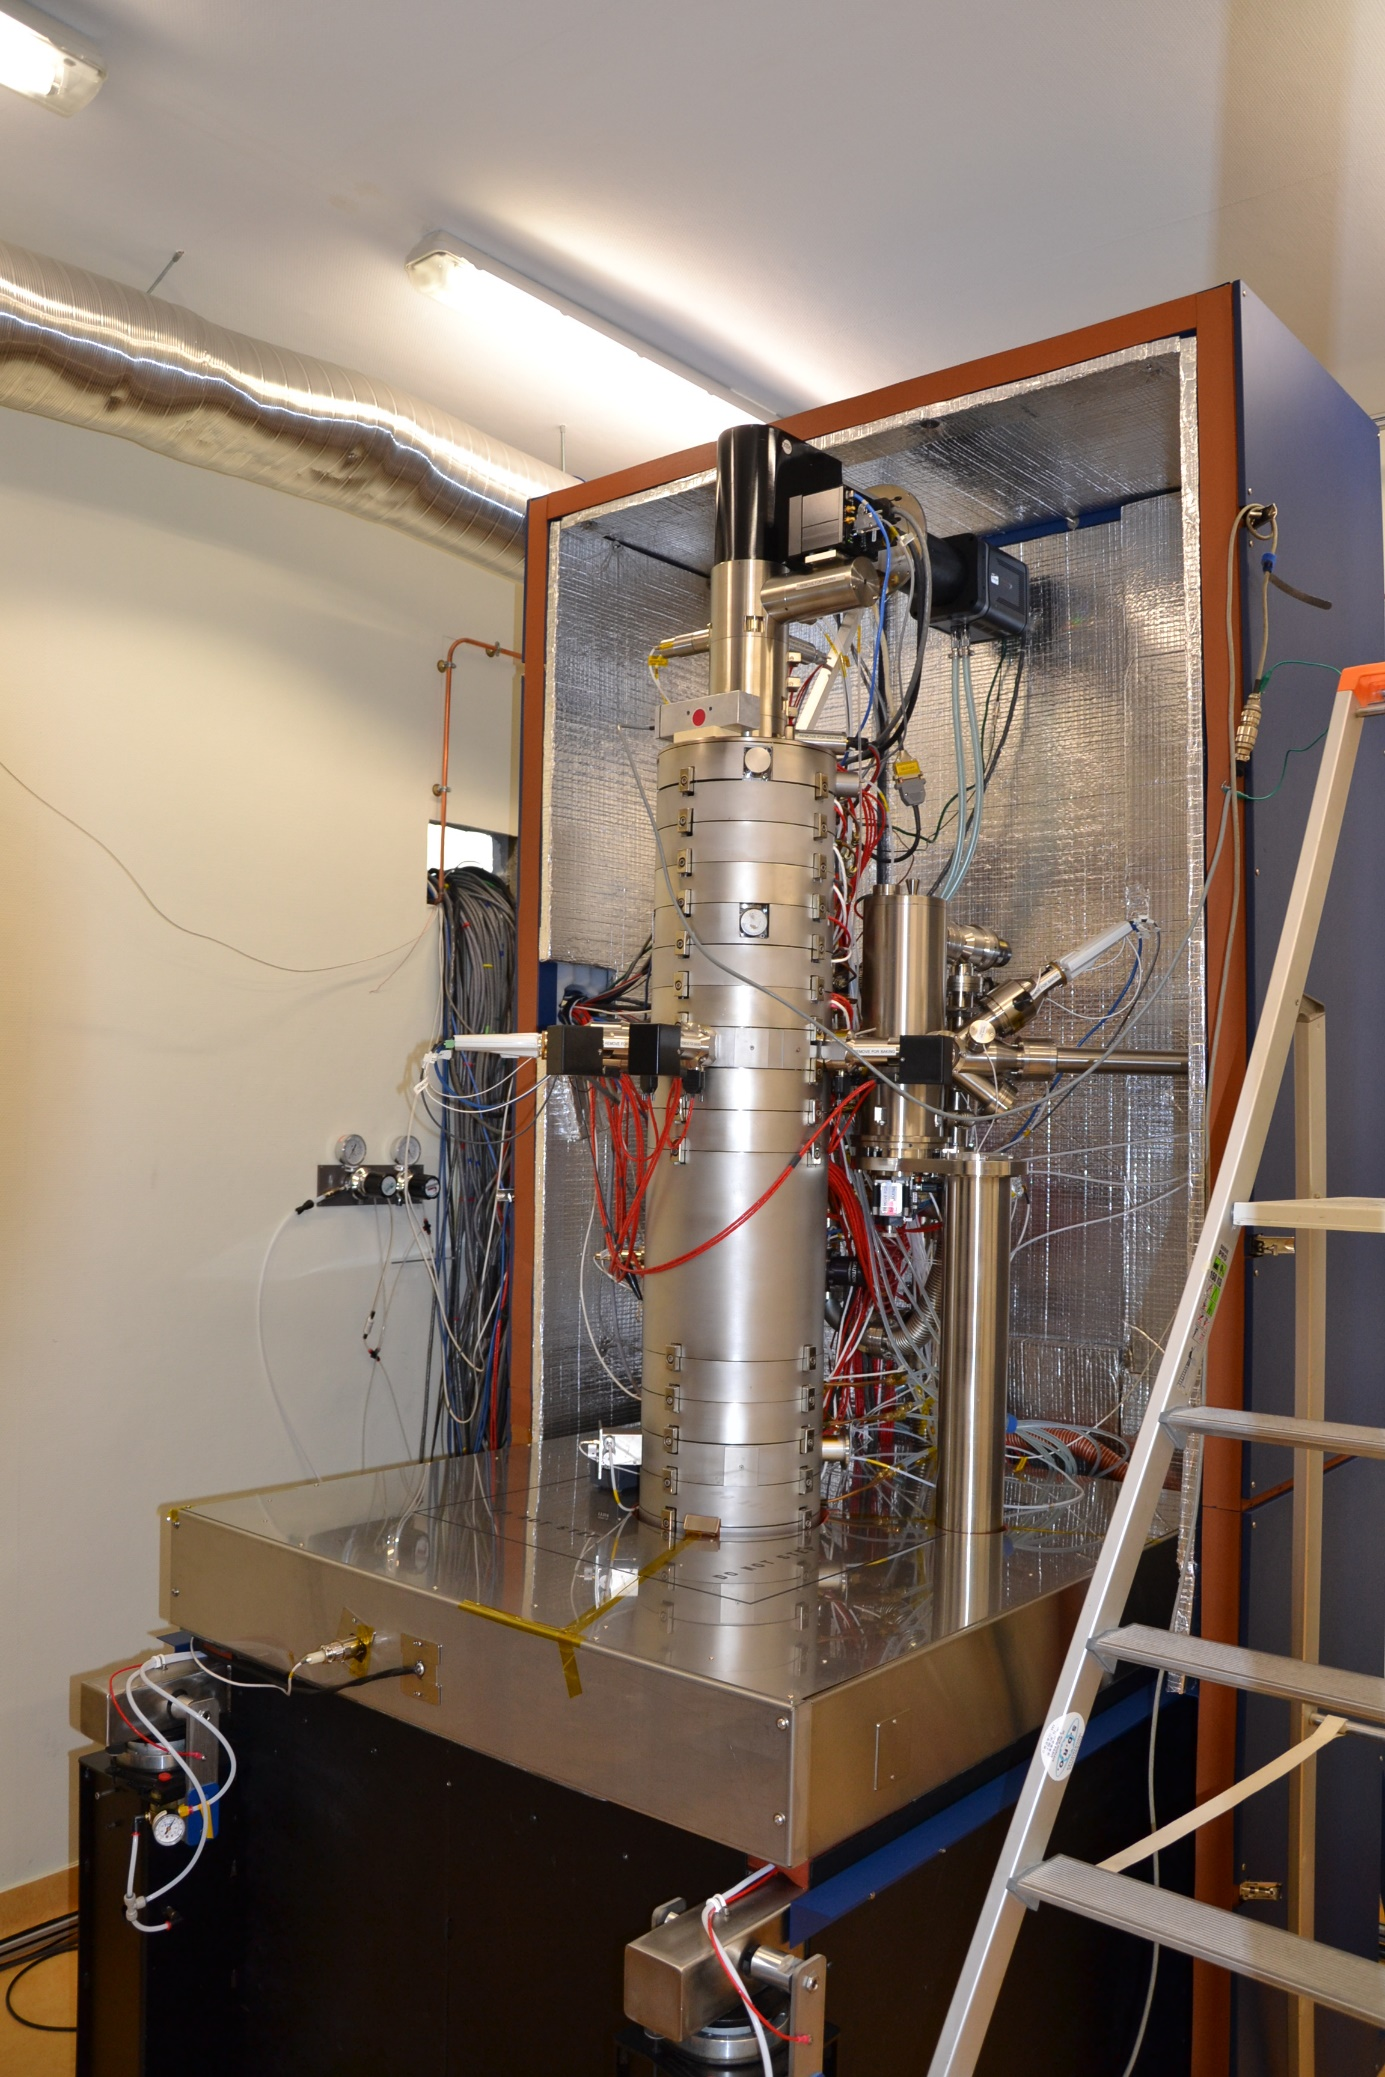
\includegraphics[width=0.4\textwidth]{img/chapitre1/figure13/NION.jpg}}
        \caption{Microscopes en service au \gls{lps} sur lesquels le mode d'acquisition aléatoire est implémenté. \subref{fig-LPS-micro-a} VG-HB501. \subref{fig-LPS-micro-b} Nion UltraSTEM 200.
            \protect\label{fig-LPS-micro}}
    \end{figure*}
    En couplant cette technique d'acquisition à des méthodes de débruitage performantes, on observe une grande amélioration de la qualité de l'acquisition, en particulier pour des temps d'exposition faibles ou des échantillons sensibles. 
    
    Cependant, la grande flexibilité du paramétrage du chemin d'acquisition ouvre la voie à une nouvelle alternative, celle d'accroître la dose d'électrons par pixel (et donc le \gls{snr} associé), mais à ne visiter qu'un nombre réduit de positions spatiales en stoppant l'acquisition aléatoire avant son terme. Un algorithme de reconstruction d'image vient enfin compléter les positions manquantes en post-traitement. En paramétrant correctement la dose d'électrons par pixels et le nombre de positions visités, la dose d'électrons utilisée est la même que pour les techniques d'acquisition standards et la dégradation de l'échantillon reste identique. 
    %
    Cette façon de procéder a motivé l'usage de techniques de reconstruction performantes issues de la communauté du traitement du signal et il s'agit d'un domaine de recherche très actif en microscopies \gls{stem}~\cite{beche2016compressed,stevens2014potential} et \gls{sem}~\cite{anderson2013sparse} entre autres.
    %
    D'autre part, les performances de cette approche sont intimement liées au choix du chemin d'acquisition et différents travaux présentés à la \cref{sec-art-micro} se sont intéressés à la part d'aléatoire et de régularité à introduire dans ce choix. Certains d'entre eux ont également proposé d'acquérir l'image partielle de manière dynamique en déterminant à chaque instant d'acquisition le pixel à visiter à l'instant suivant.
    %
    Les deux protocoles d'acquisition (débruitage et reconstruction) ont à la fois des avantages et des inconvénients. D'une manière générale, une acquisition à faible dose fournit des informations spatiales plus riches tandis que les données partiellement acquises ont un contenu spectral plus riche. Déterminer quelle approche est la meilleure n'est pas trivial et des études récentes ont comparées ces deux approches~\cite{trampert2018ultramicroscopy,sanders2020inpainting,sanders2018inpainting} en se basant sur des expériences réalisées sur des images synthétiques et réelles.
    
    Enfin, les techniques de reconstruction sont encore assez marginales dans l'équipe et n'ont été utilisées qu'en cathodoluminescence \cite{zobelli2019spatial}. 
    %
    Les efforts récents se sont concentrés sur la reconstruction en ligne du spectre-image dans une bande et sa visualisation afin de déterminer si l'élément d'intérêt est présent dans la région observée%
    %
    \footnote{%
    Il ne s'agit pas ici de reconstruire le spectre-image complet, mais seulement de sommer des bandes du spectre-image incomplet autour d'un seuil d'intérêt, puis de reconstruire l'image 2D partielle obtenue. Il ne s'agit pas d'une technique d'analyse complètement fiable puisque l'on visualise aussi les effets des seuils précédents, mais cela permet de donner une première idée quant à la présence de l'élément cherché au cours de l'acquisition.}%
    . 
    Cela permettrait d'arrêter prématurément l'acquisition si l'élément est absent, préservant ainsi l'échantillon et accélérant la recherche d'une zone d'intérêt. 
    %
    Une fois ceci fait, des techniques de reconstruction hors-ligne efficaces (et possiblement gourmandes en ressources) seraient nécessaires afin de reconstruire les spectre-images avec une grande précision. Enfin, l'échantillonnage partiel pourrait être utilisé sur les zones étudiées afin de préserver l'échantillon tout en maximisant le \gls{snr}, l'image complète étant restituée a posteriori.
    
    Le travail de thèse présenté dans ce manuscrit a pour but d'évaluer l'apport de l'échantillonnage partiel dans l'acquisition d'échantillons sensibles en imagerie STEM-EELS. Plus précisément, je m'intéresse tout particulièrement à proposer des techniques de reconstruction rapides et efficaces à mettre en \oe{}uvre au cours de l'acquisition. Celles-ci seront comparées à des méthodes de reconstruction plus longues constituant l'état de l'art. Dans ce but, le chapitre~\ref{ch-chapter_2} fera le point sur les méthodes de reconstruction d'images et sur leur utilisation dans la communauté en microscopie.
    
    
    
    
    
    

